\documentclass[main.tex]{subfiles} % Subfile-Class


% ============================================================================== %
%                            Subfile document                                    %
% ============================================================================== %

\begin{document}

% Template

\section{Liniensensor}
Anbei folgen diverse Unterkapitel, welche zur Berechnungen für die Erstellung eines Liniensensors benötigt wurden.

\subsection{Auswertung des Liniensensors}
In diesem Kapitel wird auf die Auswertung des Liniensensors eingegangen. In Abbildung~\ref{fig:Auswertung_Liniensensor} ist die
Auswertung des Liniensensors zu sehen. Hierbei wird Spannung über dem Phototransistor gemessen und mit einem ADC in einen digitalen
Wert umgewandelt. Je mehr Licht einer Emitter-Diode auf den Phototransistor reflektiert wird, desto höher ist der Strom durch ihn. Zu jedem
Zeitpunkt kann der Phototransistor als eine Stromquelle betrachtet werden. Daher ist es möglich die Spannung über ihn zu messen. Wenn der Strom
gross ist, fällt die meiste Spannung über dem Vorwiderstand ab und die Spannung über den Phototransistor nähert sich 0V an. Wenn der Phototransistor
allerdings weniger Strom "fordert", dann entsteht ein Spannungsteiler mit dem Widerstand R und dem Phototransistor. Daher ist dann die Spannung über ihn nicht in
der Nähe von 0V. Damit der Widerstand R optimal dimensioniert werden kann, muss der Strom I durch den Phototransistor in der praxis gemessen
werden. Im folgendem Kapitel wird  eruiert, mit welchem Lichtspektrum die grössere Stromdifferenz zwischen Klebeband und Fliese/ Fuge gemessen werden kann.


\begin{figure}[h!]
    \centering
    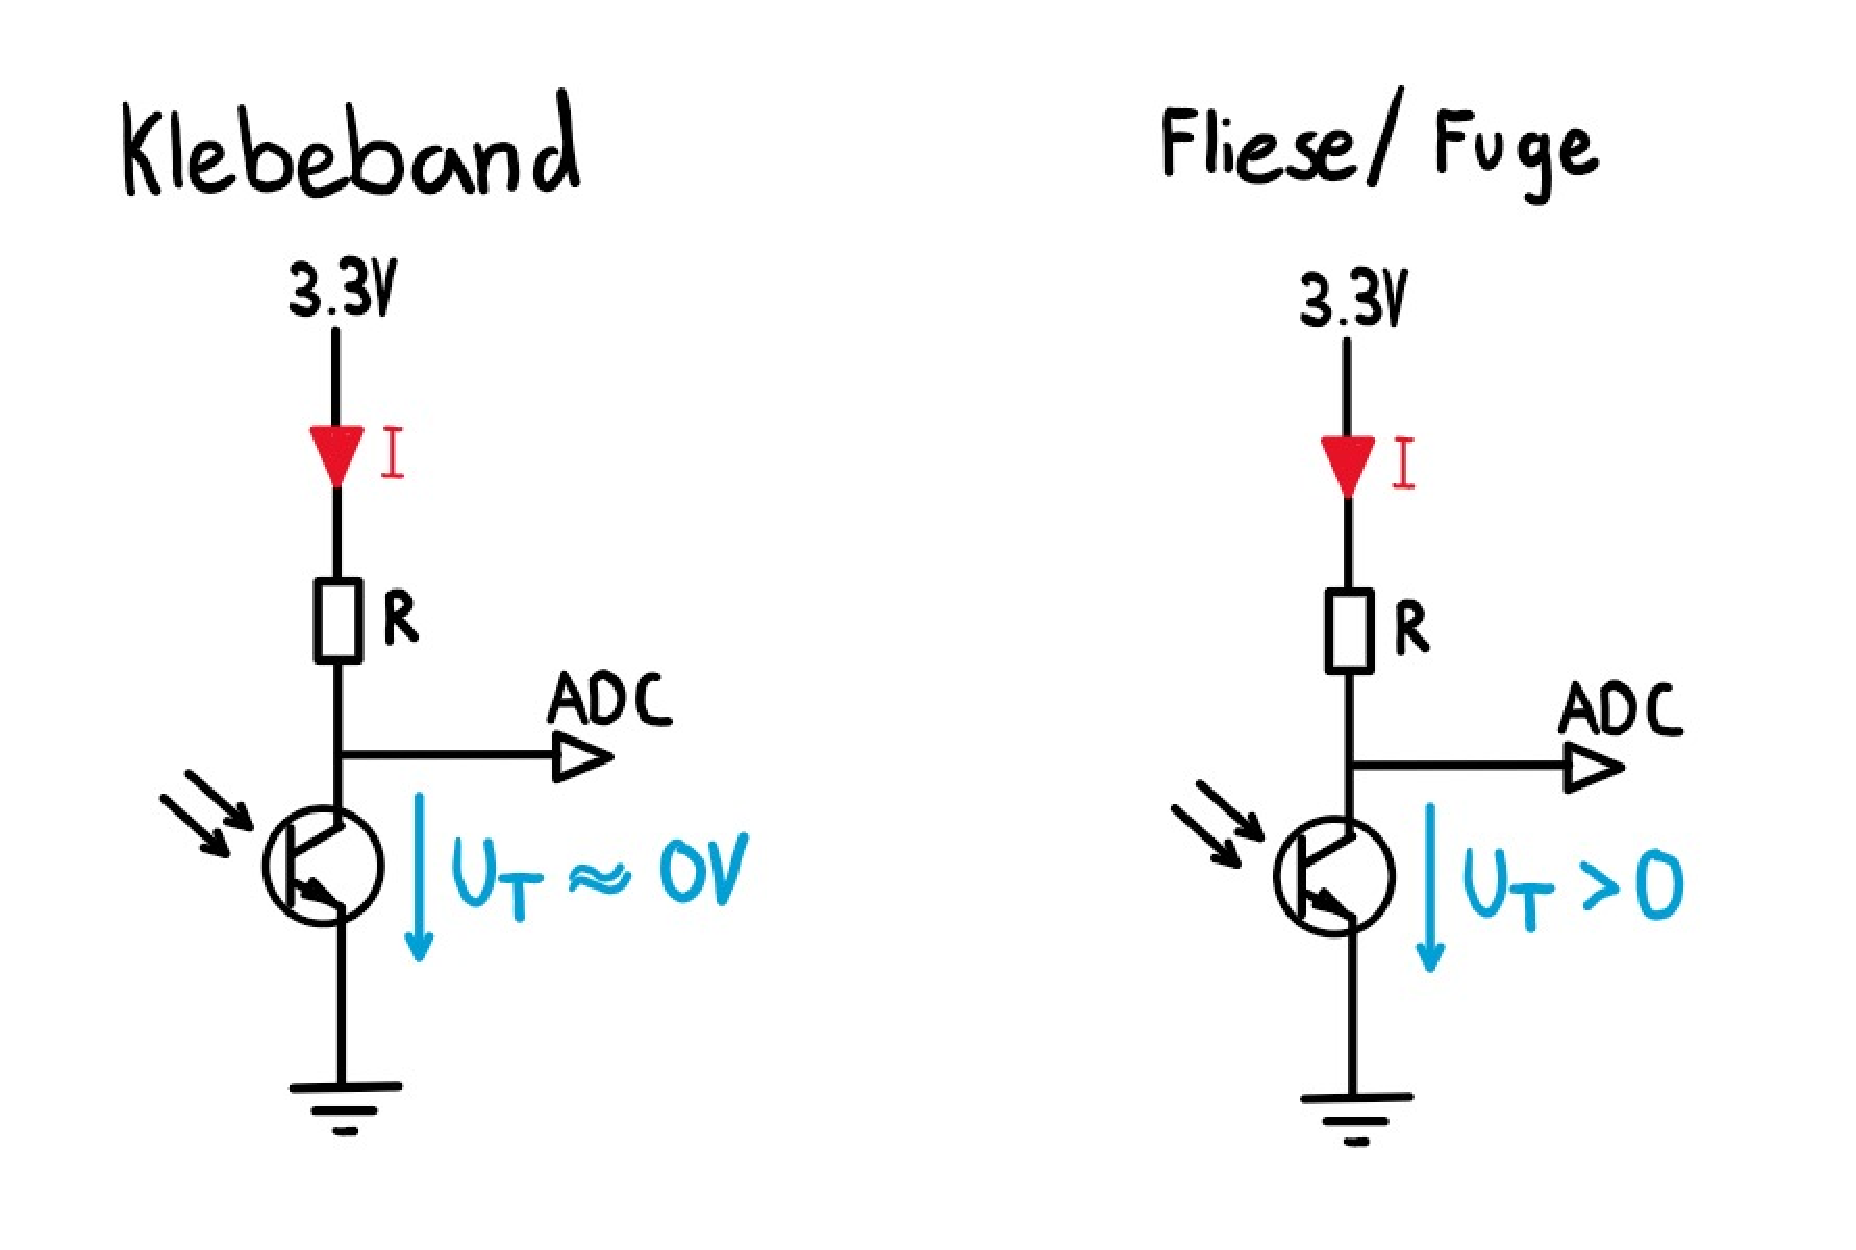
\includegraphics[width=0.5\textwidth]{./fig_Liniensensor/Auswertung_Liniensensor}
    \caption{Auswertung der Spannung über dem Phototransistor auf dem Klebeband und auf der Fliese/ Fuge.}~\label{fig:Auswertung_Liniensensor}
\end{figure}

\subsection{Analyse optimales Lichtspektrum für den Liniensensor}

Im folgendem Abschnitt wird untersucht ob sich das infrarot Spektrum oder das ultraviolette Spektrum besser für
die Unterscheidung des Klebebands zum Wettkampfuntergrund eignet. Zuerst müssen aber alle Komponenten der Messzellen, 
welche mit unterschiedlichen Wellenlängen emittierenden Dioden und Fototransistoren ausgestattet sind, berechnet werden.
In Abbildung~\ref{fig:Schema_Messzelle_Liniensensor} ist die erste Messzelle von acht abgebildet. Für jede Messzelle
gelten aber dieselben Werte.

\begin{figure}[h!]
    \centering
    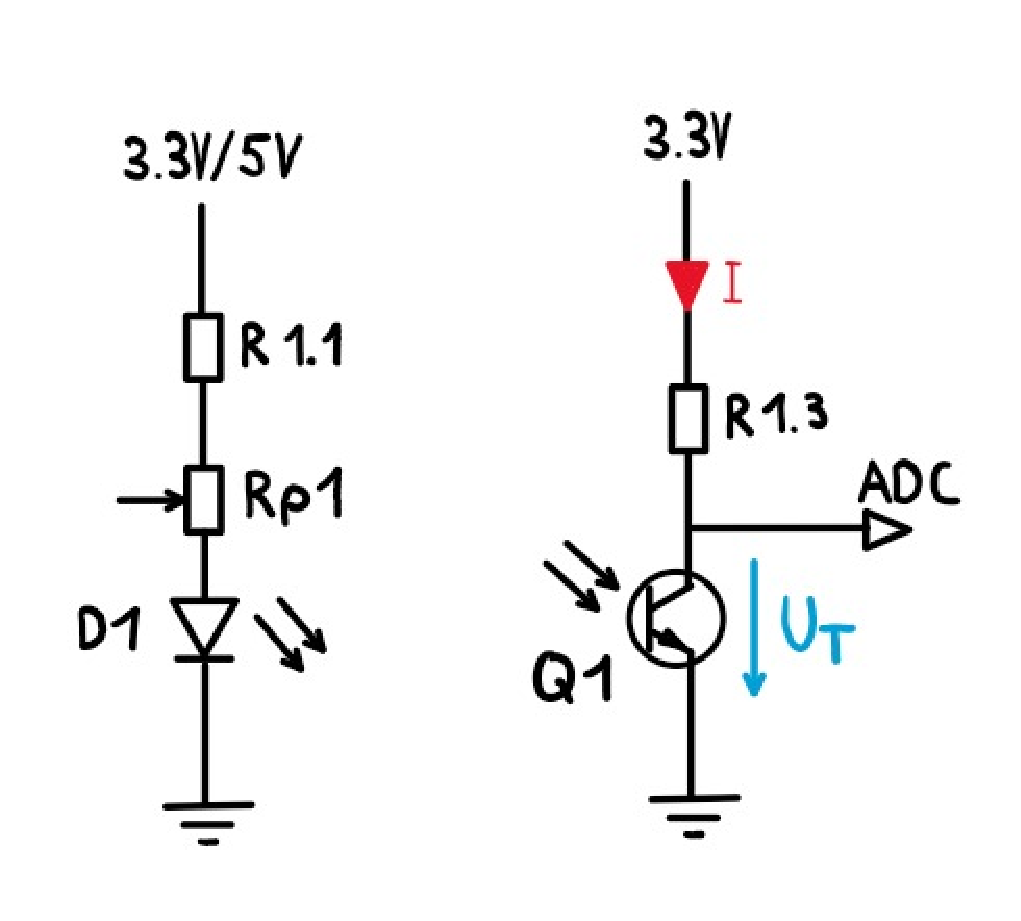
\includegraphics[width=0.5\textwidth]{./fig_Liniensensor/Schema_Messzelle_Liniensensor}
    \caption{Erste Messzelle des Liniensensors, die restlichen sieben Messzellen sind identisch.}~\label{fig:Schema_Messzelle_Liniensensor}
\end{figure}


\subsubsection{Dimensionierung IR-Messzelle}
In diesem Abschnitt wird eine IR-Messzelle dimensionert. Gemäss Datenblatt kann über dem IR-Emitter von 1.3 bis 2V
abfallen. Die Speisespannung beträgt 3.3V. Der maximaler Strom beträgt 100mA. Der Strom wird gewählt, dass er ungefähr im 
Bereich von 10mA bis 60mA fällt. Dies wurde so gewählt, das nicht zu viel Leistung verbraucht wird, aber der Emitter trotzdem 
mit genügen Strom versorgt wird. Daraus resultiert die folgende Widersandsberechnung:
\[
    R_{max} = \frac{U_q - U_{LED}}{I_{LEDmin}} = \frac{3.3V - 1.3V}{0.01A} = 200ohm
\]
\[
    R_{min} = \frac{U_q - U_{LED}}{I_{LEDmax}} = \frac{3.3V - 1.3V}{0.03A} = 33.33ohm
\]
Daraus resultiert ein Potentiometer Rp1 von 200ohm und ein R1.1 von 33ohm.

Der Widerstand R1.3 wird beim Versuch durch ein Amperemeter ersetzt, damit der Strom durch den Phototransistor gemessen 
werden kann.

%===========================================================================================================%

\subsubsection{Dimensionierung UV-Messzelle}
In diesem Abschnitt wird die UV-Messzelle dimensioniert.
Über die Speisespannung von 5V wird eine UV-Emitter mit Vorwiderstand bestromt. Der empfohlene Strom
wird Gemäss dem Datenblatt des UV-Emitters von 10mA bis 20mA vorgeschlagen. Ausserdem darf der Strom nicht 
30mA übersteigen. Daher resultiert: 

\[
    R_{max} = \frac{U_q - U_{LED}}{I_{LEDmin}} = \frac{5V - 2.9V}{0.01A} = 210ohm
\]
\[
    R_{min} = \frac{U_q - U_{LED}}{I_{LEDmax}} = \frac{5V - 2.9V}{0.03A} = 70ohm
\]
Daraus resultiert ein Potentiometer Rp1 von 200ohm und ein R1.1 von 82ohm, welches ungefähr im zuvor festgelegten
Strombereich liegt:
\[
    I_{max} = \frac{U_R}{R_{min}} = \frac{2.1}{82ohm} = 0.0256A = 25.6mA
\]
\[
    I_{min} = \frac{U_R}{R_{max}} = \frac{2.1}{282ohm} = 0.00745A = 7.45mA
\]
Aufgrund dieser Widerstandsaufteilung kann der Strom ungefähr in dem empfohlenen Bereich frei eingestellt werden.


Der Widerstand R1.3 wird beim Versuch durch ein Amperemeter ersetzt, damit der Strom durch den Phototransistor gemessen 
werden kann.

\subsubsection{Versuchsmessungen}
Bei den beiden oben dimensionierten Varianten wird je eine Messzelle auf ein PCB gelötet und dann der Strom durch den
Phototransisor gemessen. Die gemessenen Werte sind in der folgenden Tabelle~\ref{tab:Strommessungen} festgehalten. Dabei resultierte der 
Abstand von XYZ!!!!!!!!!!!!!!!!! von Messfläche zum Liniensensor. Das Potentiometer wird maximal eingestellt, sprich
auf 200 Ohm eingestellt.

\begin{table}[h]                                    
    \centering
    \begin{tabular}{|c|c|c|c|c|c|c|}                        
        \hline
        \textbf{Lichtspektrum} & \textbf{Strom Klebeband [mA]}        & \textbf{Strom Fuge [mA]}    & \textbf{Strom Fliese [mA]}\\ \hline
        Infrarot              & 1.368                                 & 1.248                        & 1.92                       \\ \hline
        Ultraviolett          & 0.2024                                & 0.0691                       & 0.0494                     \\ \hline

        \end{tabular}
\caption{Strom durch die beiden Phototransistor in verschiedenen Lichtspektren}
\label{tab:Strommessungen}
\end{table}


Aus der Tabelle ist zu sehen, dass im UV-Lichtspektrum zwar der Strom geringer ist, aber der Strom deutlich höher ist auf dem Klebeband im 
Vergleich zu den anderen Messpunkten. Daher kann die Vermutung bestätigt werden, dass das Klebeband eine fluoreszierende Wirkung hat. Aufgrund
dieser Messresultate wird auf das UV-Spektrum zurückgegriffen.


\subsection{Dimensionierung des Widerstandes R1.3}
Weil nun der Strom durch den Phototransistor bekannt ist, kann nun in diesem Abschnitt der Widerstandswert von R1.3 berechnet werden. Weil der Strom
durch den Phototransistor auf dem Klebeband nie ganz genau identisch sein wird, wird ein Schwellwert angenommen. Es wird nun ein Strom $I_{\text{Ph}}$ von $120 \, \mu A$
angenommen. Dieser Wert bietet noch genügend Differenz zum Fliesen-/Fugenstrom. Daher kann der Widerstand $R_{1.3}$ berechnet werden.

\[
    R_{1.3} = \frac{U_q}{I_{\text{Ph}}} = \frac{3.3 \, \text{V}}{120 \, \mu \text{A}} = 27.5 \, \text{k}\Omega
\]


Daraus resultiert ein Widerstand R1.3 von 27000 Ohm. Dass mit der Wahl dieses Widerstandes die Spannungsdifferenz zwischen Klebeband und Fliese/ Fuge
genügend gross ist, wird mit den folgenden Messungen in der Tabelle~\ref{tab:Spannungsmessungen} bewiesen:

\begin{table}[h]                                    
    \centering
    \begin{tabular}{|c|c|c|c|c|c|c|}                        
        \hline
             \textbf{Spannung Klebeband [V]}        & \textbf{Spannung Fuge [V]}    & \textbf{Spannung Fliese [V]}\\ \hline
             0.242                                   & 3.113                          & 2.46                       \\ \hline

        \end{tabular}
\caption{Spannung über Phototransistor bei Klebeband, Fuge und Fliese im UV-Spektrum}
\label{tab:Spannungsmessungen}
\end{table}

%===========================================================================================================%
\end{document}
